\begin{pastexam}[label={px:df3-096-ds-04}]{地方三等資訊處理 96 年 第四題}
（申論；20 分）

一個圖形 G 以節點集 V 與邊集 E 表示，邊（$u, v$）的長度以 d（$u, v$）表示。
\begin{itemize}[leftmargin=2em, labelsep=0.3em, itemsep=2pt]
\item[㈠] 設計一資料結構用以寫一段虛擬碼（psudo-code）程式描述求取 minimum cost spanning tree
的 Prim's 演算法，並說明此程式的時間複雜度（time complexity）。（10 分）
\item[㈡] 用 Prim's 演算法以節點 a 為起點逐步演算下圖的 minimum cost spanning tree。（10 分）
\end{itemize}
\begin{center}
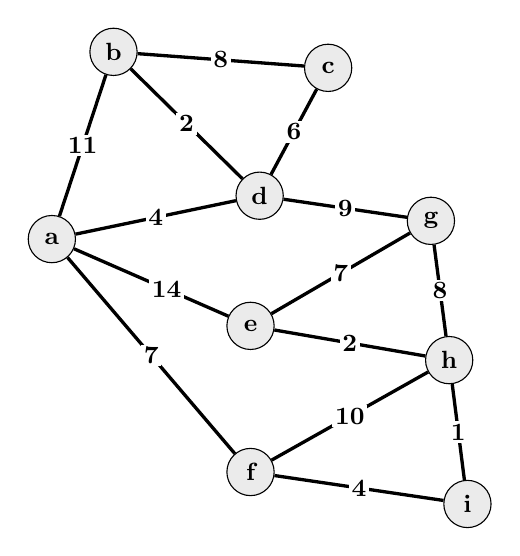
\begin{tikzpicture}[x=1.45cm, y=1.45cm,
  v/.style={circle, draw, fill=black!8, minimum size=6mm, inner sep=0pt, font=\small\bfseries},
  w/.style={fill=white, inner sep=1pt, font=\small\bfseries}]
\node[v] (b) at (1.02,-0.70) {b};
\node[v] (c) at (2.90,-0.84) {c};
\node[v] (d) at (2.30,-1.96) {d};
\node[v] (g) at (3.80,-2.18) {g};
\node[v] (a) at (0.48,-2.34) {a};
\node[v] (e) at (2.22,-3.10) {e};
\node[v] (h) at (3.96,-3.40) {h};
\node[v] (f) at (2.22,-4.38) {f};
\node[v] (i) at (4.12,-4.66) {i};
\draw[line width=1.2pt] (b)--node[w]{8}(c);
\draw[line width=1.2pt] (b)--node[w]{2}(d);
\draw[line width=1.2pt] (c)--node[w]{6}(d);
\draw[line width=1.2pt] (a)--node[w]{11}(b);
\draw[line width=1.2pt] (a)--node[w]{4}(d);
\draw[line width=1.2pt] (d)--node[w]{9}(g);
\draw[line width=1.2pt] (a)--node[w,pos=0.6]{14}(e);
\draw[line width=1.2pt] (e)--node[w]{7}(g);
\draw[line width=1.2pt] (g)--node[w]{8}(h);
\draw[line width=1.2pt] (e)--node[w]{2}(h);
\draw[line width=1.2pt] (a)--node[w]{7}(f);
\draw[line width=1.2pt] (f)--node[w]{10}(h);
\draw[line width=1.2pt] (h)--node[w]{1}(i);
\draw[line width=1.2pt] (f)--node[w]{4}(i);
\end{tikzpicture}
\end{center}
\end{pastexam}

\begin{pastsoln}
原題的「psudo-code」是 pseudo-code 的錯字，照錄。

\textbf{㈠ 資料結構。}
\begin{itemize}[nosep]
\item 圖用\textbf{相鄰串列} $\mathit{Adj}[u]$ 存：$u$ 的每個鄰居 $v$ 和長度 $d(u, v)$。
\item $\mathit{key}[v]$：目前把 $v$ 接到「已經長出來的樹」的最便宜邊的長度；$\pi[v]$：那條邊在
樹上的另一端。 $\mathit{inTree}[v]$ 記錄 $v$ 是否已經在樹上。
\item 最小優先佇列 $Q$（用二元最小堆積，以 $\mathit{key}$ 為鍵）放還沒進樹的頂點，支援
\proc{Extract-Min} 和 \proc{Decrease-Key}（堆積裡記下每個頂點的位置，才能直接找到它往上調，
資結書第~8.3~節）。
\end{itemize}
\begin{pseudo}{Prim 演算法（相鄰串列＋二元堆積）}
\Procedure{MST-Prim}{$G, d, r$}
    \For{每個頂點 $v \in V$}
        \State $\mathit{key}[v] \gets \infty$；$\pi[v] \gets \NIL$；$\mathit{inTree}[v] \gets \FALSE$
    \EndFor
    \State $\mathit{key}[r] \gets 0$
    \State 把所有頂點以 $\mathit{key}$ 為鍵放進最小堆積 $Q$
    \While{$Q$ 不是空的}
        \State $u \gets$ \Call{Extract-Min}{$Q$} \Comment{最便宜的跨越邊的端點}
        \State $\mathit{inTree}[u] \gets \TRUE$ \Comment{邊 $(\pi[u], u)$ 加入樹}
        \For{每個 $v \in \mathit{Adj}[u]$}
            \If{$\mathit{inTree}[v] = \FALSE$ \AND $d(u, v) < \mathit{key}[v]$}
                \State $\pi[v] \gets u$
                \State \Call{Decrease-Key}{$Q, v, d(u, v)$}
            \EndIf
        \EndFor
    \EndWhile
    \State \Return $\{(\pi[v], v) : v \ne r\}$
\EndProcedure
\end{pseudo}
\textbf{為什麼對}：每次取出的 $u$，$(\pi[u], u)$ 是「樹」和「樹外」之間最便宜的邊；由切割性質
（資結書定理~24.1），這條邊一定屬於某棵最小生成樹，所以一路加下去得到的是最小生成樹（資結書
第~24.3~節）。

\textbf{時間複雜度}，$n = |V|$、$m = |E|$：
\begin{itemize}[nosep]
\item 初始化和建堆積 $O(n)$。
\item \proc{Extract-Min} 做 $n$ 次，每次 $O(\lg n)$，共 $O(n \lg n)$。
\item 每條邊在兩端各被看一次，共 $2m$ 次比較；\proc{Decrease-Key} 最多 $m$ 次，每次 $O(\lg n)$。
\end{itemize}
合計 $O((n + m) \lg n) = O(m \lg n)$（連通圖 $m \ge n - 1$）。 若改用\textbf{相鄰矩陣}，
$\mathit{key}$ 用一般陣列、每次線性掃描找最小值，則是 $n$ 次 $\times$ $O(n)$，共 $O(n^2)$，
稠密圖（$m \approx n^2$）時這樣反而比較好（資結書虛擬碼~24.5）。

\textbf{㈡ 從 a 開始逐步演算。} 下表每一列是「取出最小 key 的頂點，加入對應的邊，再用它更新
鄰居的 key」之後的狀態；格子寫 key（括號裡是 $\pi$），「—」表示已經在樹上，粗體是這一步被
更新的。
\begin{center}
\small
\setlength{\tabcolsep}{3.5pt}
\begin{tabular}{ccccccccccc}
\toprule
步 & 加入 & 加入的邊 & b & c & d & e & f & g & h & i \\
\midrule
1 & a & — & \textbf{11(a)} & $\infty$ & \textbf{4(a)} & \textbf{14(a)} & \textbf{7(a)} & $\infty$ & $\infty$ & $\infty$ \\
2 & d & (a, d) 4 & \textbf{2(d)} & \textbf{6(d)} & — & 14(a) & 7(a) & \textbf{9(d)} & $\infty$ & $\infty$ \\
3 & b & (d, b) 2 & — & 6(d) & — & 14(a) & 7(a) & 9(d) & $\infty$ & $\infty$ \\
4 & c & (d, c) 6 & — & — & — & 14(a) & 7(a) & 9(d) & $\infty$ & $\infty$ \\
5 & f & (a, f) 7 & — & — & — & 14(a) & — & 9(d) & \textbf{10(f)} & \textbf{4(f)} \\
6 & i & (f, i) 4 & — & — & — & 14(a) & — & 9(d) & \textbf{1(i)} & — \\
7 & h & (i, h) 1 & — & — & — & \textbf{2(h)} & — & \textbf{8(h)} & — & — \\
8 & e & (h, e) 2 & — & — & — & — & — & \textbf{7(e)} & — & — \\
9 & g & (e, g) 7 & — & — & — & — & — & — & — & — \\
\bottomrule
\end{tabular}
\end{center}
說明幾個要注意的地方：
\begin{itemize}[nosep]
\item 第 3 步加入 b 時，b--c 的 $8$ 比 c 目前的 $6$ 大，不更新；b--a 的 a 已在樹上，不看。
\item 第 5 步可選的是 e $14$、f $7$、g $9$，取 f。 第 6 步取 i（$4 < 9 < 10 < 14$），i--h 的
$1$ 把 h 從 $10$ 降到 $1$。
\item 第 7 步加入 h 後，e 由 $14$ 降到 $2$、g 由 $9$ 降到 $8$；第 8 步加入 e，g 再降到 $7$。
\end{itemize}
每一步要取的最小值都只有一個，沒有平手。 加入順序是 a, d, b, c, f, i, h, e, g，最小生成樹的
$8$ 條邊：
\[
(a, d)\,4,\ (d, b)\,2,\ (d, c)\,6,\ (a, f)\,7,\ (f, i)\,4,\ (i, h)\,1,\ (h, e)\,2,\ (e, g)\,7,
\]
總成本 $4 + 2 + 6 + 7 + 4 + 1 + 2 + 7 = 33$。
\begin{center}
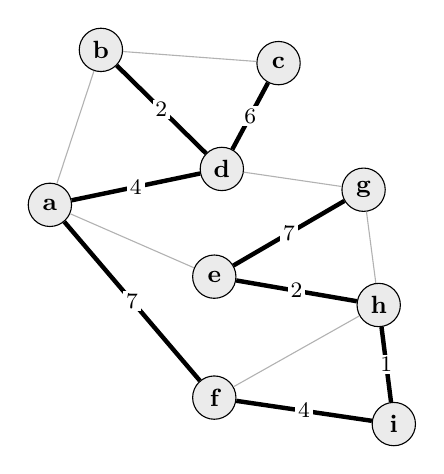
\begin{tikzpicture}[x=1.2cm, y=1.2cm,
  v/.style={circle, draw, fill=black!8, minimum size=5.5mm, inner sep=0pt, font=\small\bfseries},
  w/.style={fill=white, inner sep=1pt, font=\footnotesize}]
\node[v] (b) at (1.02,-0.70) {b};
\node[v] (c) at (2.90,-0.84) {c};
\node[v] (d) at (2.30,-1.96) {d};
\node[v] (g) at (3.80,-2.18) {g};
\node[v] (a) at (0.48,-2.34) {a};
\node[v] (e) at (2.22,-3.10) {e};
\node[v] (h) at (3.96,-3.40) {h};
\node[v] (f) at (2.22,-4.38) {f};
\node[v] (i) at (4.12,-4.66) {i};
\draw[black!30] (b)--(c) (a)--(b) (d)--(g) (a)--(e) (g)--(h) (f)--(h);
\draw[line width=1.6pt] (a)--node[w]{4}(d);
\draw[line width=1.6pt] (b)--node[w]{2}(d);
\draw[line width=1.6pt] (c)--node[w]{6}(d);
\draw[line width=1.6pt] (a)--node[w]{7}(f);
\draw[line width=1.6pt] (f)--node[w]{4}(i);
\draw[line width=1.6pt] (h)--node[w]{1}(i);
\draw[line width=1.6pt] (e)--node[w]{2}(h);
\draw[line width=1.6pt] (e)--node[w]{7}(g);
\end{tikzpicture}
\end{center}
粗線是最小生成樹，淺色是沒選的邊。 用 Kruskal 檢查：依序 $1, 2, 2, 4, 4, 6, 7, 7$ 都不成環，
第 $9$ 條起（$8, 8, 9, \ldots$）都會成環，同樣得到總成本 $33$。
\end{pastsoln}
